\documentclass{../template/Report}%方括号内写yuxi即生成预习报告\documentclass[yuxi]{../template/Report}
\settemplatedir{../template/}%设置模板路径

\exname{惠斯登电桥} %实验名称
\extable{} %实验桌号
\instructor{} %指导教师
\class{} %班级
\name{} %姓名
\stuid{} %学号

\nyear{} %年
\nmonth{} %月
\nday{} %日
\nweekday{} %星期几,e.g. \nweekday{三}
\daypart{}%上午/下午

\redate{} %如有实验补做,补做日期
\resitu{} %情况说明:

\begin{document}
\maketitle

\section{预习报告(10分)}
(注:将已经写好的“物理实验预习报告”内容拷贝过来)

\subsection{实验综述(5分)}
(自述实验现象、实验原理和实验方法,包括必要的光路图、电路图、公式等。不超过500字。)

如图所示,$R_1$、$R_2$、$R_s$ 和 $R_x$ 联成一四边形 ACBD,每条边为电桥的一个桥臂。在测量过程中调节 $R_1$、$R_2$ 和 $R_s$ 使检流计中没有电流通过,即“桥”的两端 C 和 D 两点电位相等,这时称为电桥平衡。此时 $R_2 R_x = R_s R_1$,即
\[
    R_x = \frac{R_1}{R_2} R_s
\]
\begin{figure}[H]
    \centering
    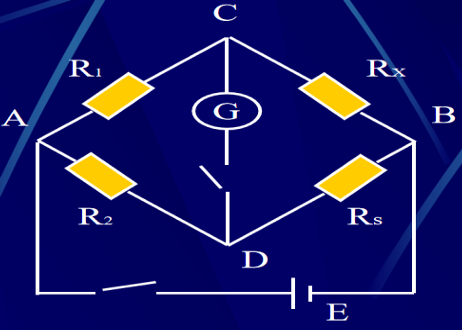
\includegraphics[width=0.6\textwidth]{电桥.png}
    \caption{惠斯登电桥实验电路图}
    \label{fig:电桥}
\end{figure}
当电表平衡后,若微小改变被测电阻值,检流计的指针并不发生偏转,显然这时它没有反映被测电阻的这一改变,那么改变多大的阻值时它才能反映呢?这与电桥的灵敏度有关,为了定量的确定电桥灵敏度,其定义为:
\[
    S = \frac{\Delta N}{\Delta R_x} = \frac{\Delta N}{R}
\]
式中 $\Delta N$ 为发生 $\Delta R_x$ 或 $\Delta R$ 时检流计偏转的格数。由于 $\Delta R_x$ 或 $\Delta R/R$ 为相对改变之值,故上式又有相对灵敏度之称,$S$ 越大,说明电桥越灵敏,测量误差越小。

如\cref{fig:电桥}所示自组电桥,设电桥的灵敏度足够高,考虑到 $R_1$、$R_2$、$R_s$ 的自身误差,此时相对不确定度为:
\[
    \frac{\Delta R_x}{R_x} = \sqrt{ \left(\frac{\Delta R_1}{R_1}\right)^2 + \left(\frac{\Delta R_2}{R_2}\right)^2 + \left(\frac{\Delta R_s}{R_s}\right)^2 }
\]
其中 $\Delta R_1$, $\Delta R_2$, $\Delta R_s$ 分别为 $R_1$, $R_2$, $R_s$ 的不确定度。为了尽量减小系统误差,可将 $R_1$ 和 $R_2$ 互换位置,设 $R_s$ 变为 $R_s'$ 时电桥重新达到平衡,这时有 $R_x = \frac{R_2}{R_1} \cdot R_s'$,得
\[
    R_x = \sqrt{R_s R_s'}
\]

这样就消除了由 $R_1$ 和 $R_2$ 自身的误差对 $R_x$ 所引入的测量误差,求出 $R_x$ 的相对不确定度为
\[
    \frac{\Delta R_x}{R_x} = \frac{1}{2}\left[\left(\frac{\Delta R_s}{R_s}\right)^2+\left(\frac{\Delta R_s}{R_s}\right)^2\right]^{\frac{1}{2}} = \frac{\Delta R_s}{R_s}
\]
它只与 $R_s$ 的仪器误差有关。而 $R_s$ 可选用具有一定精度的标准电阻箱,这样的 $R_x$ 的系统误差就可减小。实验时 $R_s$ 常用十进位转盘直流电阻箱,其仪器允差为
\[
    \frac{\Delta R_s}{R_s} = \pm \left( a + b \frac{m}{R_s} \right) \%
\]
其中 $R_s$ 是电阻箱的指示值,$a$ 是电阻箱的精确度等级,$b$ 是与精确度等级有关的系数,$m$ 为所使用电阻箱的总盘数。一般常用的 0.1 级十进位转盘电阻箱 $a=0.1$,$b=0.2$,则
\[
    \Delta R_s = \pm (0.001 R_s + 0.002 m)
\]

\subsection{实验重点(3分)}
(简述本实验的学习重点,不超过100字。)
\begin{enumerate}
    \item 掌握惠斯登电桥工作原理及其特点,学会自组电桥测量未知电阻。
    \item 掌握正确使用盒式惠斯登电桥测量电阻的方法。
    \item 学习如何对测量结果进行误差分析。
\end{enumerate}
\subsection{实验难点(2分)}
(简述本实验的实现难点,不超过100字。)
\begin{enumerate}
    \item  检流计上的“电计”与“短路”按钮都具有锁定功能,测量时要确保“短路”按钮未锁
    定,否则检流计不会有偏转。
    \item 使用盒式惠斯登电桥,在电桥未平衡时,G键只能瞬间按下,待指针一偏转应立即放开G
    键。
    \item 实验结束,关闭检流计和盒式惠斯登电桥。
\end{enumerate}

\begin{fullreportonly}
\section{原始数据(20分)}
(将有老师签名的“自备数据记录草稿纸”的扫描或手机拍摄图粘贴在下方,完整保留姓名,学号,教师签字和日期。)
\begin{figure}[H]
    \centering
    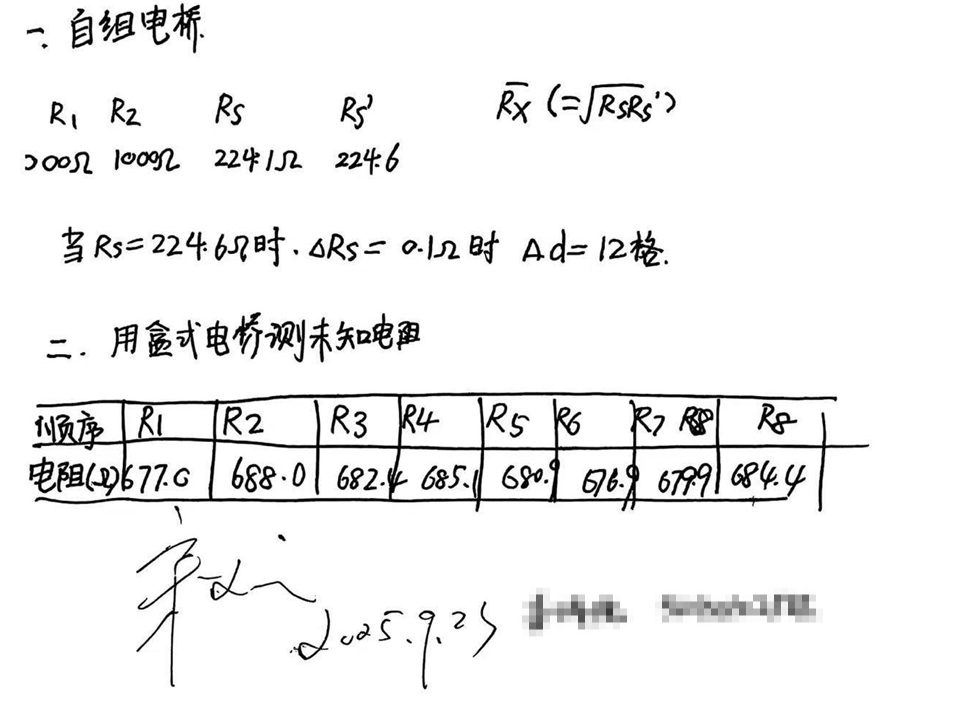
\includegraphics[width=0.8\textwidth]{数据.png}
    \caption{原始数据记录}
    \label{fig:原始数据}
\end{figure}
\section{结果与分析(60分)}
\subsection{数据处理与结果(30分)}
(列出数据表格、选择适合的数据处理方法、写出测量或计算结果。)
\subsubsection{自组电桥测量未知电阻}
\begin{table}[H]
    \centering % 使表格居中
    \caption{测量得到的数据}
    \begin{tabular}{|C{0.08\textwidth}|C{0.08\textwidth}|C{0.08\textwidth}|C{0.08\textwidth}|C{0.08\textwidth}|C{0.08\textwidth}|C{0.08\textwidth}|}
        \hline
        % 表头
        $R_1$ / \si{\ohm} & $R_2$ / \si{\ohm} & $R_s$ / \si{\ohm} & $R_s'$ / \si{\ohm} & $R_x$ / \si{\ohm} & $\Delta R_s'$ / \SI{0.1}{\ohm} & $\Delta d$ / 格 \\
        \hline
        % 数据行
        1000 & 1000 & 224.1 & 224.6 & 224.3 & 0.1 & 12 \\
        \hline
    \end{tabular}
\end{table}
\[
    S = \frac{\Delta d}{\frac{\Delta R_s}{R_s}} = \frac{12}{\frac{0.1}{224.6}} = 26952
\]

$R_x$ 相对不确定度
\[
    E = \frac{\Delta R_x}{R_x} = \sqrt{\left(\frac{\Delta R_s}{R_s}\right)^2 + \left(\frac{\Delta S}{S}\right)^2} = \sqrt{\left(0.001 + \frac{0.002m}{R_s}\right)^2 + \left(\frac{0.2}{S}\right)^2} = 0.001
\]

则 $\Delta R_x = E \cdot \overline{R_x} = \SI{0.224}{\ohm}$,则 $\overline{R_x} = \sqrt{R_s R_s'} = \SI{224.3}{\ohm}$。

则 $R_x = (\overline{R_x} \pm \Delta R_x)\,\si{\ohm} = (224.3 \pm 0.224)\,\si{\ohm}$。
\subsubsection{用盒式惠斯登电桥测量未知电阻}
\begin{table}[H]
    \centering
    % \caption{表格标题}
    \begin{tabular}{|C{0.1\textwidth}|C{0.08\textwidth}|C{0.08\textwidth}|C{0.08\textwidth}|C{0.08\textwidth}|C{0.08\textwidth}|C{0.08\textwidth}|C{0.08\textwidth}|C{0.08\textwidth}|}
        \hline
        待测电阻 & $R_1$ & $R_2$ & $R_3$ & $R_4$ & $R_5$ & $R_6$ & $R_7$ & $R_8$ \\
        \hline
        电阻(\si{\ohm}) & 677.0 & 688.0 & 682.4 & 685.1 & 680.9 & 676.9 & 679.9 & 684.4 \\
        \hline
    \end{tabular}
\end{table}

\[
    \overline{R_x} = \frac{1}{8}\sum_{i=1}^{8} R_{xi} = \SI{681.8}{\ohm}, \quad \text{标准偏差} S = \sqrt{\frac{1}{8-1}\sum_{i=1}^{8}(R_{xi} - \overline{R_x})^2} = \SI{3.9}{\ohm}
.\]

\[
    \text{离散度} = \frac{S}{\overline{R_x}} \times 100\% = 0.57\%
.\]

\subsection{误差分析(20分)}
(运用测量误差、相对误差或不确定度等分析实验结果,写出完整的结果表达式,并分析误差原因。)
\begin{enumerate}
    \item  人在肉眼观察检流计指针是否指零时,存在\textbf{视觉误差}。
    \item 桥臂电阻的误差,电桥中\textbf{四个桥臂电阻的标称值与实际值之间存在偏差}。即使使用高精度
        电阻,也存在微小的容差。计算公式$R_x = \frac{R_1}{R_2} R_3$是理想情况,如果$R_1, R_2, R_3$本
        身不准,计算出的$R_x$也必然不准。
    \item 有时按下“电计”按钮,已完成调零,再松开时发现又\textbf{发生微小偏转},这给$R_s$和$R_s'$的测量结果带来误差。
    \item \textbf{实验中电阻箱$R_s$的分度值为$0.1\si{\ohm}$},在实际测量时,电阻箱变化$1.0\si{\ohm}$时,\textbf{检流计从左偏可能会变为右偏},这给$R_s$和$R_s'$的测量结果带来误差。
\end{enumerate}
\subsection{实验探讨(10分)}
(对实验内容、现象和过程的小结,不超过100字。)

在惠斯登电桥实验中,我们亲自动手连接电路,并通过调节电阻使检流计指零来测定未
知阻值。实验采用的交换测量法有效降低了系统误差。整个过程深化了对电桥平衡原理的理
解,并锻炼了不确定度评估与有效数字处理的数据分析能力。
\section{思考题(10分)}
(解答教材或讲义或老师布置的思考题,请先写题干,再作答。)
\subsection{为什么用惠斯登电桥测电阻比伏安法测量的准确度高?用电桥法测电阻产生误差的主要因素是什么?}

\subsubsection{准确高的原因}
\begin{enumerate}
    \item \textbf{测量原理优势:} 惠斯登电桥基于平衡原理,当电桥平衡时,检流计中无电流通过,此时被测电阻与标准电阻之间存在精确的比例关系,(其中,$R_1$为比率臂电阻,$R_2$为标准电阻),测量结果仅依赖于标准电阻和比率臂的精度,而非电流、电压的直接测量量。

    \item \textbf{消除系统误差:} 伏安法需同时测量电流和电压,电表的内阻会引入系统误差(如电流表分压、电压表分流),无论采用内接法还是外接法,都无法完全消除电表内阻的影响;而电桥法在平衡时无需直接测量电流或电压,避免了电表内阻的影响。

    \item \textbf{灵敏度特性:} 电桥的灵敏度可通过调节参数(如电源电压、检流计灵敏度)提高,从而更精确地判断平衡状态,减小读数误差。

    \item \textbf{电源稳定性:} 对电源稳定性要求不高。电源电压的波动会影响桥路失衡时的电流,但一旦调节到平衡点(检流计指零),电源电压的变化不会改变平衡条件。
\end{enumerate}
\subsubsection{用电桥法测电阻产生误差的主要因素}
\begin{enumerate}
    \item \textbf{桥臂电阻的误差:}测量结果$ R_x = \frac{R_1}{R_2} \cdot Rs $的精度直接依赖于三个已知电阻$R_1, R_2, R_s$的精度。如果这些电阻的标称值不准、随时间漂移或因温度变化而改变,会直接导致系统误差。
    \item \textbf{电桥的灵敏度带来的误差:}如果电桥灵敏度不够高,当检流计指针指在“零”位时,
        桥路可能并未完全平衡,只是失衡电流太小以至于检流计无法检测到。这个无法被察
        觉的微小失衡就会带来误差。
    \item \textbf{热效应:}电流流过电阻时会产生热量,导致电阻值发生变化(尤其是标准电阻和待测
        电阻)。如果电桥不平衡时通过$R_x$和$R_s$的电流过大,可能会因发热而改变其阻值,
        即使后来调至平衡,测得的也已不是常温下的阻值。
    \item \textbf{人为操作误差:}调节电阻箱时判断平衡点不准确。
\end{enumerate}
\subsection{为了提高电桥测量灵敏度,应采取哪些措施?为什么?}
\subsubsection{具体措施}
\begin{enumerate}
    \item 在允许范围内增大电源电压,可增加电桥回路的电流,使不平衡时检流计的偏转幅度增
    大,灵敏度提高。但需注意被测电阻的功率限制,避免过热损坏
    \item 使比率臂$\frac{R_1}{R_2}$的取值接近1,此时电桥对电阻变化的灵敏度最高。
    \item 选用最小分度值小的电阻箱
\end{enumerate}
\subsubsection{原因}
电桥的灵敏度本质上取决于“单位电阻变化引起的检流计偏转量”。电源电压升高或检流计灵
敏度提高,会直接放大信号输出;比率臂接近1时,电桥处于最敏感状态,此时被测电阻的
微小变化会导致检流计明显偏转;而减小附加电阻可使测量更接近理想状态,避免灵敏度被
额外损耗。
\subsection{用电桥测电阻时,若线路接通后检流计指针总是往一个方向偏转或总不偏转,试分析是什么原因?}
\subsubsection{总是往一个方向偏转}
可能是电桥的比率臂(倍率)选择不合理,导致偏差过大(比率臂与标准电阻$R_s$的乘积远大于或小于被测电阻$R_x$);也可能是电路连接有误,出现了短路或断路。
\subsubsection{总不偏转}
可能是电路连接有误,如电桥回路中某处(如导线、开关、电阻)完全断开或检流计本身被短路;也可能是电源未接通或仪器本身出现故障。
\subsection{惠斯登电桥比率臂选取的原则是什么?为什么要这样选取?}
\subsubsection{原则}
\begin{enumerate}
    \item 使标准电阻$R_s$的调节范围覆盖被测电阻;
    \item 尽量使比率臂接近1;
    \item 考虑标准电阻的精度等级。
    \item 在保证电阻箱不超过其最大允许电流或功率的前提下,应尽可能多地使用其有效位数(即
        从最高档位开始调节),从而提高测量结果的有效数字位数。
\end{enumerate}
\subsubsection{原因}
比率臂的选择直接影响标准电阻的调节范围和电桥灵敏度。若比率臂与$R_x$不匹配,可能导致$R_s$无法调节至平衡(如量程不足),或因灵敏度太低而无法精确读数。
接近1的比率臂能使电桥处于最佳测量状态,减少因原理导致的误差。
\subsection{如何使用自组电桥测量电表内阻(注意电表所能允许通过的最大电流)?根据电桥平衡的特点,可否将桥路中的检流计去掉,换成行测电表判别电桥的平衡?}

\begin{enumerate}
    \item \textbf{电路设计:} 自组惠斯登电桥,将被测电表(如电流表 G)接入待测臂($R_x$ 位置),注意电表的最大电流限制,需在电路中串联保护电阻 $R_p$,避免电流过大损坏电表。标准电阻臂 $R_s$ 选用可调电阻箱,比率臂 $R_1$、$R_2$ 选用高精度固定电阻或可调电阻。

    \textbf{限流保护:} 根据电表的最大允许电流 $I_g$,计算保护电阻 $R_p$ 的最小值:
    \[
        R_p \ge \frac{U}{I_g} - R_g
    \]
    电压,$R_g$ 为电表内阻估计值),确保通电后电流不超过量程。

    \textbf{调节平衡:} 接通电源,缓慢调节标准电阻 $R_s$ 和比率臂(若比率臂可调),观察电表指针的变化(或串联一个小量程电流表监测电流),当电桥平衡时,电表两端电压为零,通过电表的电流也为零(或电流无变化),此时
    \[
        \frac{R_1}{R_2} = \frac{R_x}{R_s}
    \]

    \item \textbf{理论可行性:} 电桥平衡的本质是桥路两端电势相等,此时桥路中电流为零。若将检流计换成行测电表(如电压表或电流表),当电桥平衡时,行测电表的读数应为零(或无变化),因此可通过行测电表是否示零来判断平衡。

    \textbf{但存在实际限制:}

    \textbf{灵敏度问题:} 行测电表的灵敏度通常低于专用检流计,可能无法检测到微小的不平衡电流,导致测量误差增大。

    \textbf{内阻影响:} 行测电表(如电压表)的内阻并非无穷大,接入桥路后会改变桥路的等效电阻,可能影响电桥的平衡条件,尤其是当电表内阻与桥臂电阻可比拟时,误差更明显。
\end{enumerate}
\end{fullreportonly}
\insertnotes
\end{document}